% =====================================================================
% VERSION ENSAE, REDUCTION SFE : chapitre 8, identification partielle et bornes de capital.
% Phase 3 : copie a texte constant de chapitres/10_identification_partielle.tex.
% Phase 4 (1er octobre 2026) : reecrit et condense ; formules, tableaux, figures, renvois,
% citation et nombres conserves. Le texte d'origine reste dans chapitres/ (version Institut)
% et dans l'historique Git.
% Lu par main_ensae.tex seul : ne jamais le faire lire par main_institut.tex,
% qui garde chapitres/.
% Scripts : 30 (bornes), 31 (comparaison des regimes), 33 (relatif/absolu), 34, 61, 67.
% =====================================================================
\chapter{Identification partielle et bornes de capital}
\label{chap:partielle}

Nous faisons varier le sens des liens à fréquence, sévérité et partie symétrique fixées.
Le diagnostic utilise la cascade indépendante du tableau~\ref{tab:lecture-mecanismes}, avec son
calage propre. La chaîne reste incident, perte, somme annuelle, quantile. La plage des quantiles
ainsi obtenus, conditionnelle aux liens posés, ne constitue pas un intervalle de confiance.

\section{Modèle en couches}

Le socle, indépendant de $W$, regroupe la fréquence d'entrée surdispersée, l'accumulation par cause
commune et la sévérité GPD. Sans contagion ($W = 0$), le besoin de capital est de $5\,275$~M\euro{} dans le calage
de référence (sévérité OpRisk, fréquence de l'état conforme, gain de propagation $g=0{,}90$).

Nous séparons la force commune que nous maintenons fixe et le sens que nous faisons varier.
Cela revient à décomposer la matrice de façon unique :
\[
  W \;=\; S + A, \qquad S = \tfrac{1}{2}(W + W^{\top}), \qquad A = \tfrac{1}{2}(W - W^{\top}) .
\]
Le signe de $A_{jk}$ indique le sens dominant de la paire : positif pour $j\to k$, négatif pour
$k\to j$. Sous amorce uniforme et faible intensité, les co-occurrences renseigneraient $S$ au
premier ordre, sans identifier $A$ (proposition~\ref{prop:nonid}). Faute de panel, $S$ vient du
barème d'expert et seul $A$ varie, dans l'ensemble admissible
\[
  \mathcal{W}(t) \;=\; \bigl\{\, S + A \;:\; A^{\top} = -A, \;\; |A_{jk}| \leq t\,S_{jk},
  \;\; \rho(S+A) < 1 \,\bigr\},
\]
où la contrainte $|A_{jk}| \leq S_{jk}$ découle des conditions de positivité $W_{jk}\geq 0$ et
$W_{kj}\geq 0$. Le paramètre $t\in[0,1]$ est un rayon d'ambiguïté posé qui limite l'asymétrie admise, l'ignorance
totale $t=1$ correspondant aux sources publiques actuelles. Pour chacune des $10$ paires de piliers,
$A_{jk}/S_{jk}$ varie donc entre $-t$ et $t$ : les contraintes de signe définissent un pavé,
intersecté avec la contrainte spectrale. Ses $2^{10} = 1\,024$ sommets fixent chaque paire à un
extrême : la force totale de la paire est conservée, mais placée entièrement dans un sens.
Pour chacun, nous construisons $W$, contrôlons son admissibilité, calculons la loi des
ensembles de piliers atteints, puis simulons les pertes annuelles et leur quantile. Les sommets
recensent des directions extrêmes de liens, pas des permutations ou des trajectoires d'incidents.

% SOURCES-SCRIPTS: 31 30

\section{Capital sur l'ensemble admissible}

La plage calculée aux sommets va du minimum au maximum sur les sommets admissibles, notés $V(1)$.
$\widehat B$ désigne le quantile estimé par simulation. Ces extrema ne constituent pas des bornes globales démontrées sur $\mathcal W(1)$. À $t=1$, on obtient
\[
  \left[\min_{W\in V(1)}\widehat{B}(W),\max_{W\in V(1)}\widehat{B}(W)\right] \;=\; [\,6\,858 \;;\; 8\,697\,]~\text{M\euro{}} ,
\]
avec un facteur $1{,}27$ entre les deux bouts. La contagion ajoute entre $+30\,\%$ et
$+65\,\%$ au socle. Le point d'expert, $8\,110$~M\euro{}, n'est qu'un point de cet ensemble
(figure~\ref{fig:pave-sommets}).

\begin{figure}[H]
  \centering
  \figover{Z_pave_sommets.png}
  \caption{Le pavé admissible et le capital qu'il donne. (a)~Coupe sur deux des dix paires :
$A_{jk}/S_{jk}$ va de $-1$, tout de $k$ vers $j$, à $+1$, tout de $j$ vers $k$. (b)~Capital aux
$1\,024$ sommets et aux $3\,000$ points intérieurs, à $t = 1$ : aucun point intérieur testé ne sort
de l'intervalle des extrema aux sommets.}
  \label{fig:pave-sommets}
\end{figure}

Les sommets ne bornent le capital que si les extrêmes y sont atteints, ce que rien ne garantit
\emph{a priori}. Augmenter $A_{jk}$ élève $W_{jk}$ mais abaisse $W_{kj}$, si bien que la
réponse n'est pas monotone en $A_{jk}$. Les $3\,000$ points intérieurs tirés uniformément restent tous
dans cette plage, en VaR comme en perte moyenne.

Une recherche de contre-exemples n'en trouve pas : la
perte moyenne lissée est un polynôme de degré deux en chaque coordonnée, et $172$ ascensions depuis des
sommets et des points intérieurs finissent toutes sur un sommet. Cette propriété reste vérifiée
numériquement, mais non démontrée. Ces extrema numériques sont des quantiles de $40\,000$ années simulées. À indice de queue élevé, la VaR est peu sensible à la structure de
cascade, la queue annuelle étant dominée par une perte unique. La perte moyenne, bornée
dans $[849\,;1\,100]$~M\euro{} et moins bruitée, et l'ordre de remédiation en rendent mieux compte.

Le recalcul des $1\,024$ sommets sur quatre graines donne des largeurs de $1\,461$ à
$1\,871$~M\euro{}, de moyenne $1\,739$ et d'écart-type $189$~M\euro{}. Les écarts-types des
minima et maxima sont respectivement $166$ et $186$~M\euro{}. Chaque graine sélectionne à nouveau
les extrema sur toute la grille ; leurs matrices changent. Ces dispersions mesurent le bruit de
Monte-Carlo à paramètres fixés, sans constituer un intervalle de confiance de calibration. Les
quatre répétitions ne suffisent pas à estimer finement ce bruit ; la plage historique est conservée.
% SOURCES-SCRIPTS: 134

Ramener l'ignorance de $t=1$ à $t=0{,}5$, c'est-à-dire borner l'asymétrie à la moitié de la
co-occurrence, réduirait la largeur de la plage de $1\,839$ à $695$~M\euro{}, soit $-62\,\%$. Ce scénario donne l'ordre de grandeur de ce que le reporting de la section~\ref{ch:livrable} permettrait de gagner, sans le garantir.

% SOURCES-SCRIPTS: 30 61 127

\section{Comparaison d'une matrice posée et de l'identification partielle}

\begin{center}\footnotesize
\renewcommand{\arraystretch}{1.3}
\begin{tabular}{@{}p{4.1cm} p{4.5cm} p{5.6cm}@{}}
\toprule
 & \textbf{Régime A : on pose $W$} & \textbf{Régime B : modèle en couches} \\
\midrule
Sortie sur le capital & un point, $8\,110$~M\euro{} & socle : $5\,275$ ; capital total aux sommets : $[6\,858\,;8\,697]$ \\
Part insensible au sens & aucune, tout repose sur le classeur & $79\,\%$ (socle $61\,\%$, plancher commun aux sommets $18\,\%$), à $S$ posé \\
Panel biaisé & déplace le besoin de capital de $777$~M\euro{} & la bande ne bouge pas si $S$ reste fixé \\
Priorité de remédiation & P1, sans marge d'erreur & tête P1/P4, ordre interne ouvert \\
Si aucun expert ne répond & plus de matrice complète & exploration conditionnelle au $S$ d'expert maintenu \\
\bottomrule
\end{tabular}
\end{center}

\vspace{2pt}
\noindent Faire varier la direction posée à dire d'expert, depuis un panel qui confirmerait le classeur
jusqu'à un panel qui dirait l'inverse au bord du pavé admissible, déplace le besoin de capital du
régime~A de $777$~M\euro{}, soit $10\,\%$. La priorité bascule alors entre trois piliers, sans signal
pour l'utilisateur. La bande du régime~B ne bouge pas à $S$ fixé. Le regret d'une remédiation est son gain manquant par rapport au meilleur choix sous une même matrice ; le minimax retient le plus petit regret maximal parmi les matrices testées.

Sur $150$ matrices admissibles tirées au hasard, P5 n'arrive jamais
en tête, P3 dans moins de $10\,\%$ des cas, et P1 ($45\,\%$) et P4 ($36\,\%$) concentrent $81\,\%$ des
tirages. Un panel d'experts servirait donc à départager
P1 et P4 et à resserrer la bande ; le questionnaire diffusé est resté sans réponse.

% SOURCES-SCRIPTS: 31

\section{Niveaux et rapports de capital}

\begin{center}\footnotesize
\renewcommand{\arraystretch}{1.25}
\begin{tabular}{@{}p{4.3cm} r r r r@{}}
\toprule
\textbf{Calibration} & \textbf{socle} & \textbf{bornes} &
\textbf{haute/socle} & \textbf{\% insensible au sens} \\
\midrule
Référence (OpRisk)   & $5\,275$  & $[6\,858\,;8\,697]$   & $1{,}65$ & $78{,}9\,\%$ \\
Sévérité PRC         & $239$     & $[336\,;424]$         & $1{,}77$ & $79{,}2\,\%$ \\
Fréquence $\times 3$ & $11\,709$ & $[14\,353\,;17\,405]$ & $1{,}49$ & $82{,}5\,\%$ \\
\bottomrule
\end{tabular}
\end{center}

\vspace{2pt}
\noindent La borne haute explorée varie d'un facteur $41$ entre PRC et fréquence triplée, sans
rapport uniforme entre tous les niveaux de capital. Les rapports varient d'au plus $33\,\%$ de
leur moyenne. Le moins stable, largeur de bande sur socle ($32{,}9\,\%$), diminue quand la fréquence
augmente : la queue annuelle est alors moins dominée par une perte unique. Les trois calibrations
conservent l'ordre de grandeur des rapports au socle et P1 et P4 en tête, non le niveau du capital
(figure~\ref{fig:partielle}).
% SOURCES-SCRIPTS: 33

\section{Échelle de repli sur la direction}
\label{sec:echelle-u}

On peut écrire la direction par l'excès de propagation propre à la source,
$\operatorname{logit}p_{ij}=\operatorname{logit}p_j+u_{ij}$ ($p_j$ mesure l'attractivité de la cible
$j$), puis limiter $u$ par structures successives, jusqu'à la variante sans asymétrie où $u=0$.
Une direction de rang $1$ capte $74\,\%$ de la
variance de la direction posée et resserre les bornes de $25\,\%$, au prix d'une
hypothèse de structure. Elle n'a qu'un facteur de source et un facteur de cible, donc une seule valeur singulière non nulle de $u$ (figure~\ref{fig:echelle-repli}b). Sans asymétrie,
P1 et P4 deviennent indiscernables (gains de remédiation $1\,051$ contre $1\,052$~M\euro{}),
alors que $353$~M\euro{} les séparent avec la direction du barème d'expert. C'est donc la direction qui
départage les deux piliers prioritaires.

% Largeur d'appel reduite de 1,14 a 1,04 \textwidth (au lieu de \figover) : sous le tectonic
% macOS, la figure 8.3 passait seule a la page suivante (151 pages au lieu de 150 sous Windows,
% meme source). Aucun texte ni aucune valeur ne change.
\begin{figure}[H]\centering
\makebox[\textwidth][c]{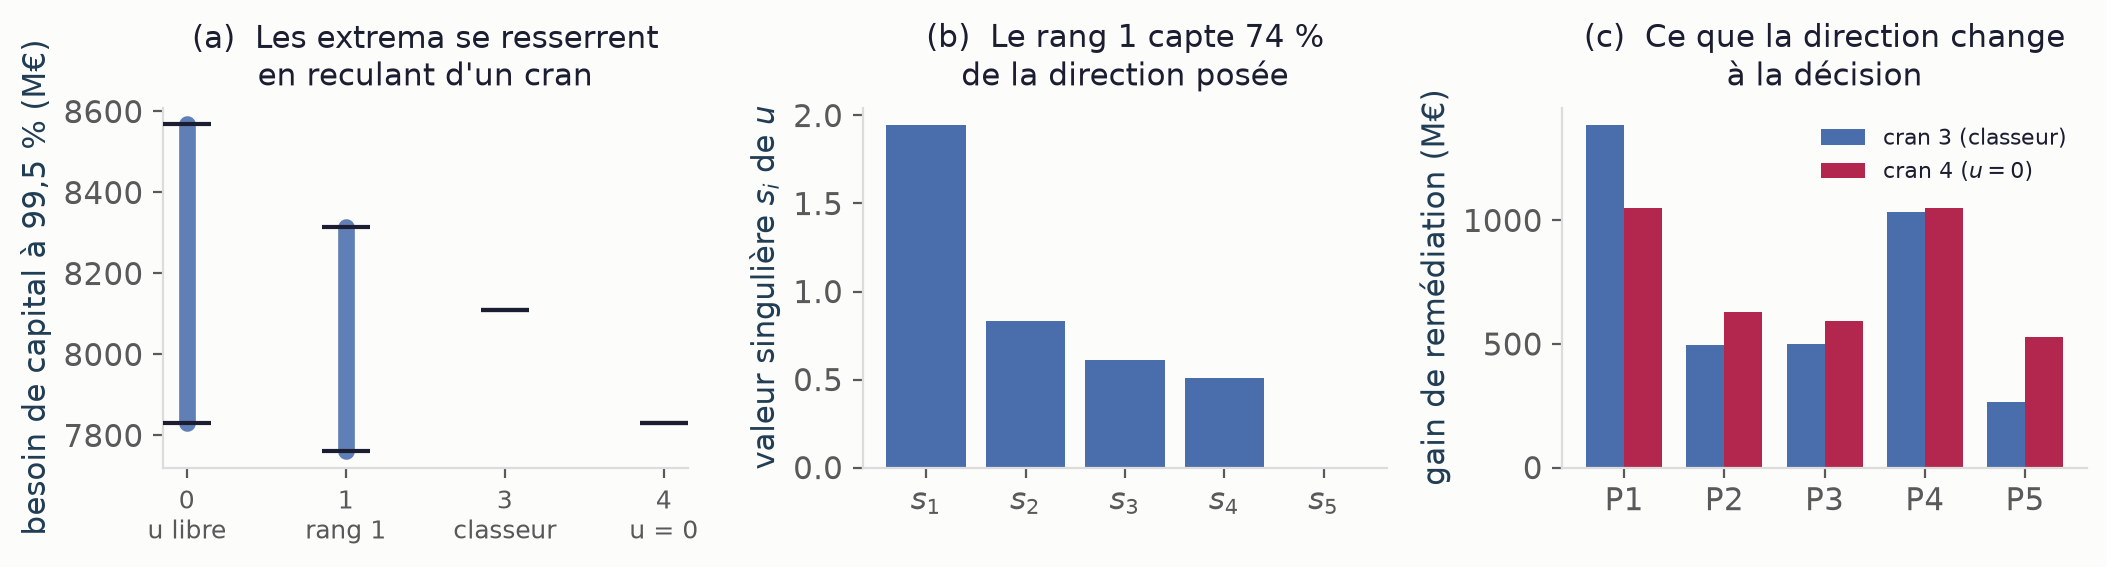
\includegraphics[width=1.04\textwidth]{Z5_echelle_repli.png}}
\caption{Échelle de repli sur la direction. (a)~Les extrema du capital aux sommets se resserrent quand la
structure est restreinte : $u$ libre, rang~$1$, barème d'expert, puis absence d'asymétrie ($u=0$). (b)~Valeurs
singulières de la direction posée : le rang~$1$ en capte l'essentiel. (c)~Gains de remédiation par
pilier avec la direction du barème d'expert et sans asymétrie.}
% SOURCES-SCRIPTS: 34
\label{fig:echelle-repli}
\end{figure}

\begin{figure}[H]
  \centering
  \makebox[\textwidth][c]{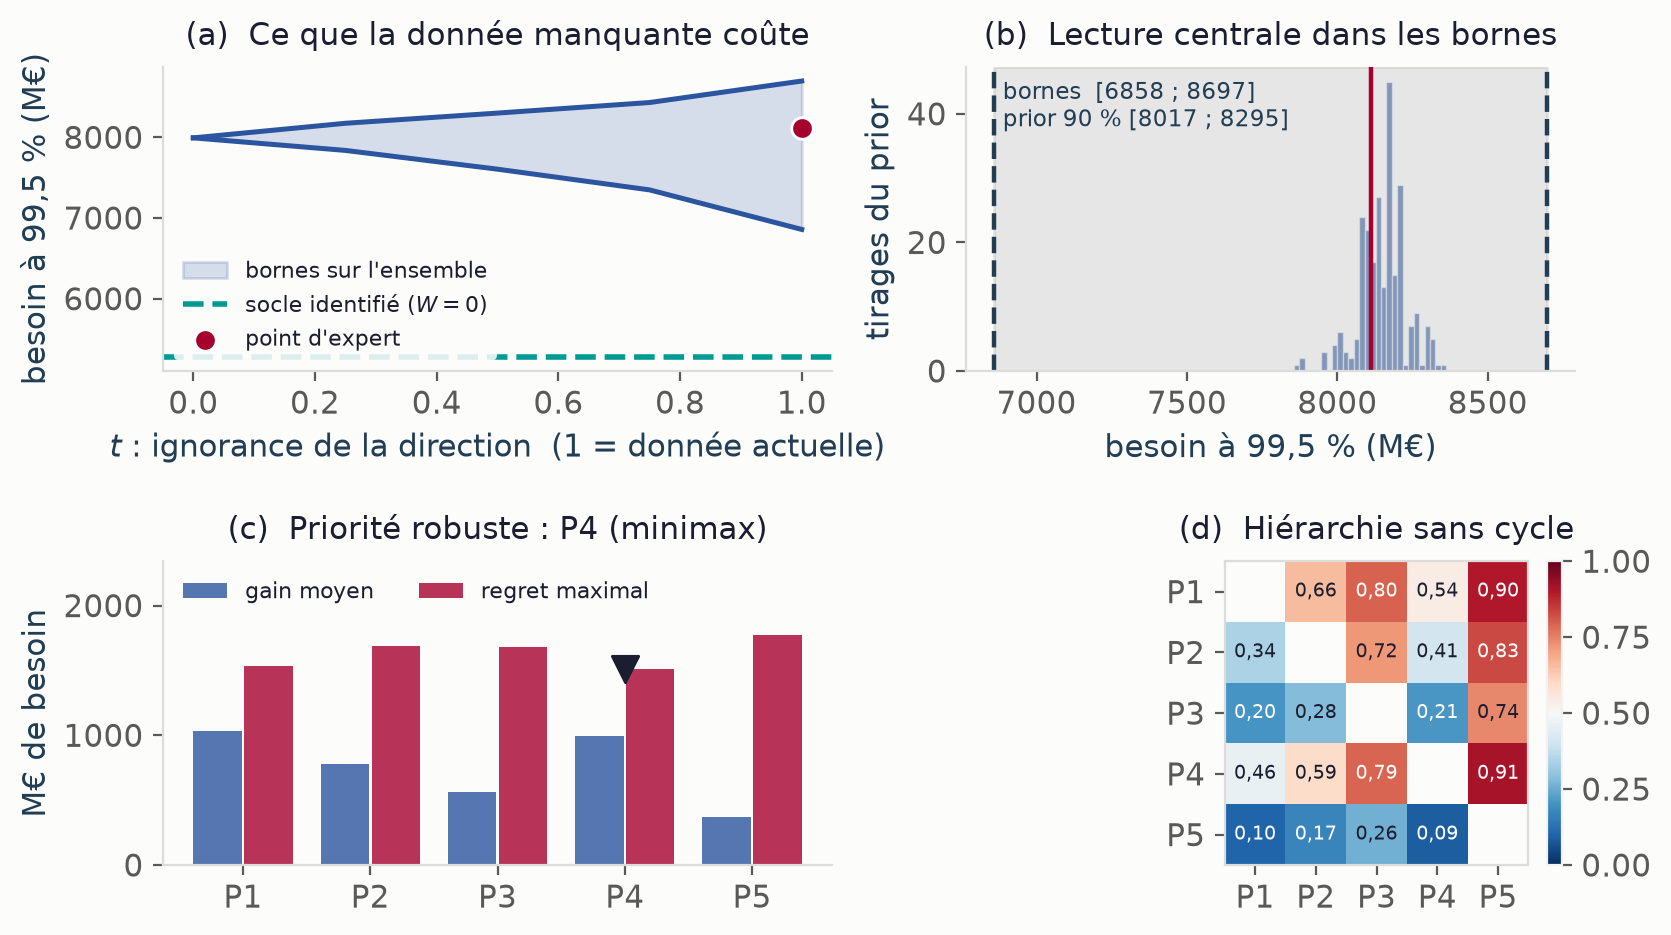
\includegraphics[width=1.04\textwidth]{Z_identification_partielle.png}}
  \caption{Identification partielle de la contagion dirigée. (a)~Les bornes se resserrent quand
l'ignorance directionnelle $t$ diminue. (b)~Le prior d'expert dans des bornes indépendantes du
choix de direction, conditionnelles à la partie symétrique posée. (c)~Priorité de remédiation (regret maximal). (d)~Dominance des
piliers sur des matrices admissibles tirées : P5 n'y arrive jamais en tête, et P1 et P4 concentrent $81\,\%$ des
matrices testées.}
  \label{fig:partielle}
\end{figure}
% SOURCES-SCRIPTS: 30 67

% SOURCES-SCRIPTS: 34

Cette plage exprime ce que le sens des liens change, à force fixée, dans la cascade indépendante.
Les écarts entre états du chapitre~\ref{chap:resultats} reposent sur la marche auto-évitante et ses
canaux ; ils ne se déduisent pas de cette plage.
